\documentclass[12pt, letterpaper]{article}

\usepackage{amsmath, enumerate, graphicx}
\allowdisplaybreaks[1]
%\usepackage[showframe]{geometry}
\usepackage{layout}
\DeclareMathOperator*{\argmin}{argmin}
\DeclareMathOperator*{\argmax}{argmax}
\newcommand{\bv}[1]{\mathbf{#1}}

\title{CS 676\\ Problem Set 1a}

\author{Josh Wheeler, Yotam Barnoy}

\setlength{\voffset}{-0.75in}
\setlength{\headsep}{5pt}
\setlength{\hoffset}{-0.5in}
\setlength{\textwidth}{450pt}

\begin{document}%\layout

\maketitle

\setcounter{section}{1}

\newcommand{\Qdef}[1][i]{\prod_{{#1}} Q_i (X_i)}

\section{Variational Inference on a Simple Network}
\subsection{Empirical Questions}
\begin{enumerate}[a.]
\item 
    \begin{align*}
        &X \in \{A,B,C,D,E,F\}\\
        &\text{minimize KL} (Q || P) = \sum_{x \in X} Q(X) \log \frac{Q(X)}{P(X)}\\
        &= \sum_{x \in X} \Qdef \log (\Qdef) - \sum_{x \in X} \Qdef \log P(x)\\
        &= \sum_{x \in X} \Qdef \sum_k \log(Q_k(X_k)) - \sum_{x \in X} \Qdef \log P(x)\\
        &= \sum_{X_j} \sum_{X_{-j}} Q_j(X_j) \Qdef[i \neq j][log Q_j(X_j) + \sum_{k \neq j} Q_k(X_k)]\\*
          &\qquad {} - \sum_{X_j} \sum_{X_{-j}} Q_j(X_j) \Qdef[i \neq j] \log P(x)\\
        &= \sum_{X_j} Q_j(X_j) \sum_{X_{-j}} \Qdef_[i \neq j] [\log Q_j(X_j) + \sum_{k \neq j} Q-K(X_k)] \\*
            &\qquad {} - \sum_{X_j} Q_j(X_j) \sum_{X_{-j}} \Qdef [i \neq j] \log P(x)\\
        &\text{Distribute:}\\*
        &= \sum_{X_j} Q_j(X_j) \sum_{X_{-j}} (\Qdef [i \neq j]) \log Q_j(X_j)
        + \sum_{X_j} Q_j(X_j) \sum_{X_{-j}} (\Qdef [i \neq j]) \sum_{k \neq j} Q_k(X_k)\\*
            &\qquad {} - \sum_{X_j} Q_j \sum_{X_{-j}} (\Qdef [i \neq j]) log P(x)\\
        &\text{Pull out constants:}\\
        &= \sum_{X_j} Q_j(X_j) \log Q_j(X_j) \sum_{X_{-j}} (\Qdef [i \neq j]) 
        + (\sum_{k \neq j} Q_k(X_k)) \sum_{X_j} Q_j(X_j) \sum_{X_{-j}}(\Qdef [i \neq j]\\*
            &\qquad {} - \sum_{X_j} Q_j(X_j)[\sum_{X_{-j}} (\Qdef[i \neq j]) \log P(x)]\\
        &\text{Drop terms that equal 1 and re-arrange:}\\
        &= \sum_{X_j} Q_j(X_j) \log Q_j(X_j) 
          - \sum_{X_j}Q_j(X_j)[\sum_{X_{-j}}(\Qdef[i \neq j]) \log P(x)]
          + \sum_{k \neq j} Q_k(X_k)\\
        &\text{Note: we let } f = \sum_{X_{-j}}(\Qdef[i \neq j]) \log P(x)\\
        &= \sum_{X_j} Q_j(X_j) \log Q_j(X_j) \sum_{x_j} Q_j(X_j) \log (\exp(f))\\
        &= \text{KL}(Q_j(X_j)||\exp f)
    \end{align*}
    Which is minimized when $Q_j = \exp f$. (We will normalize after all updates)

\item Mean field is a very crude approximation for the original distribution. We note that the KL divergence is very high ($0.829$), indicating that our approximate distribution is a bad choice.
\item The derivation for structured mean field is the same as the one above, except that we set $X = \{ABC, DEF\}$.
\item Structured mean field inference is a far better approximation for our original distribution. The KL divergence is much lower than in the previous case ($0.002$), indicating the closeness of the approximation. Additionally, the values in the approximate marginal multinomial distribution are within roughly $0.01$ of the true distribution.

Mean field inference makes many independence assumptions missing from the original model. Structured mean field inference does this a lot less.
\end{enumerate}

\setcounter{section}{4}
\section{Blocked Gibbs}
\subsection{Derivation}
    We want to compute\\
    \begin{equation*}
        P(Z_{d,i}=k, X_{d,i}=0 | Z-Z_{d,i}, X-X_{d,i}, C, W, \alpha, \beta, \lambda)
        = \frac{P(Z_{d,i}=k, X_{d,i}=0, Z-Z_{d,i}, \ldots )}
            {P(Z-Z_{d,i}, X-X_{d,i}, C, \ldots) }
    \end{equation*}
    We have a factored form for this given by equation 13.\\
    All terms that do not depend on $Z_{d,i}$ and $X_{d,i}$ will appear in both the numerator and denominator, so they cancel out.\\
    Using $a,b,c,d$ from equation 16 and 15:\\
    \begin{equation*}
        = \frac{a^{X_{d,i}=0}}{b^{X_{d,i}=0}}\frac{c^{X_{d,i}=0}}{d^{X_{d,i}=0}}(1 - \lambda)
    \end{equation*}
    Similarly for $x=1$:\\
    \begin{equation*}
        = \frac{a^{X_{d,i}=1}}{b^{X_{d,i}=1}}\frac{c^{X_{d,i}=1}}{d^{X_{d,i}=1}}(\lambda)
    \end{equation*}

\newpage
\section{Text Analysis with MCLDA}
\subsection{Empirical Questions}
\begin{enumerate}[1.]
    \item 
        We observe that all three graphs are very similar. No matter the random starting point, we still converge to a similar log likelihood for both the test and train data. 

        The shape of both the train and test curves is similar: we observe a generally increasing pattern approaching an asymptote. The two curves do differ in magnitude significantly though. The training data has much lower likelihood because it has more data, causing more probabilities to be multiplied together.

        \begin{figure}[ht]
            \caption{Train vs Test data log-likelihood, run 1}
            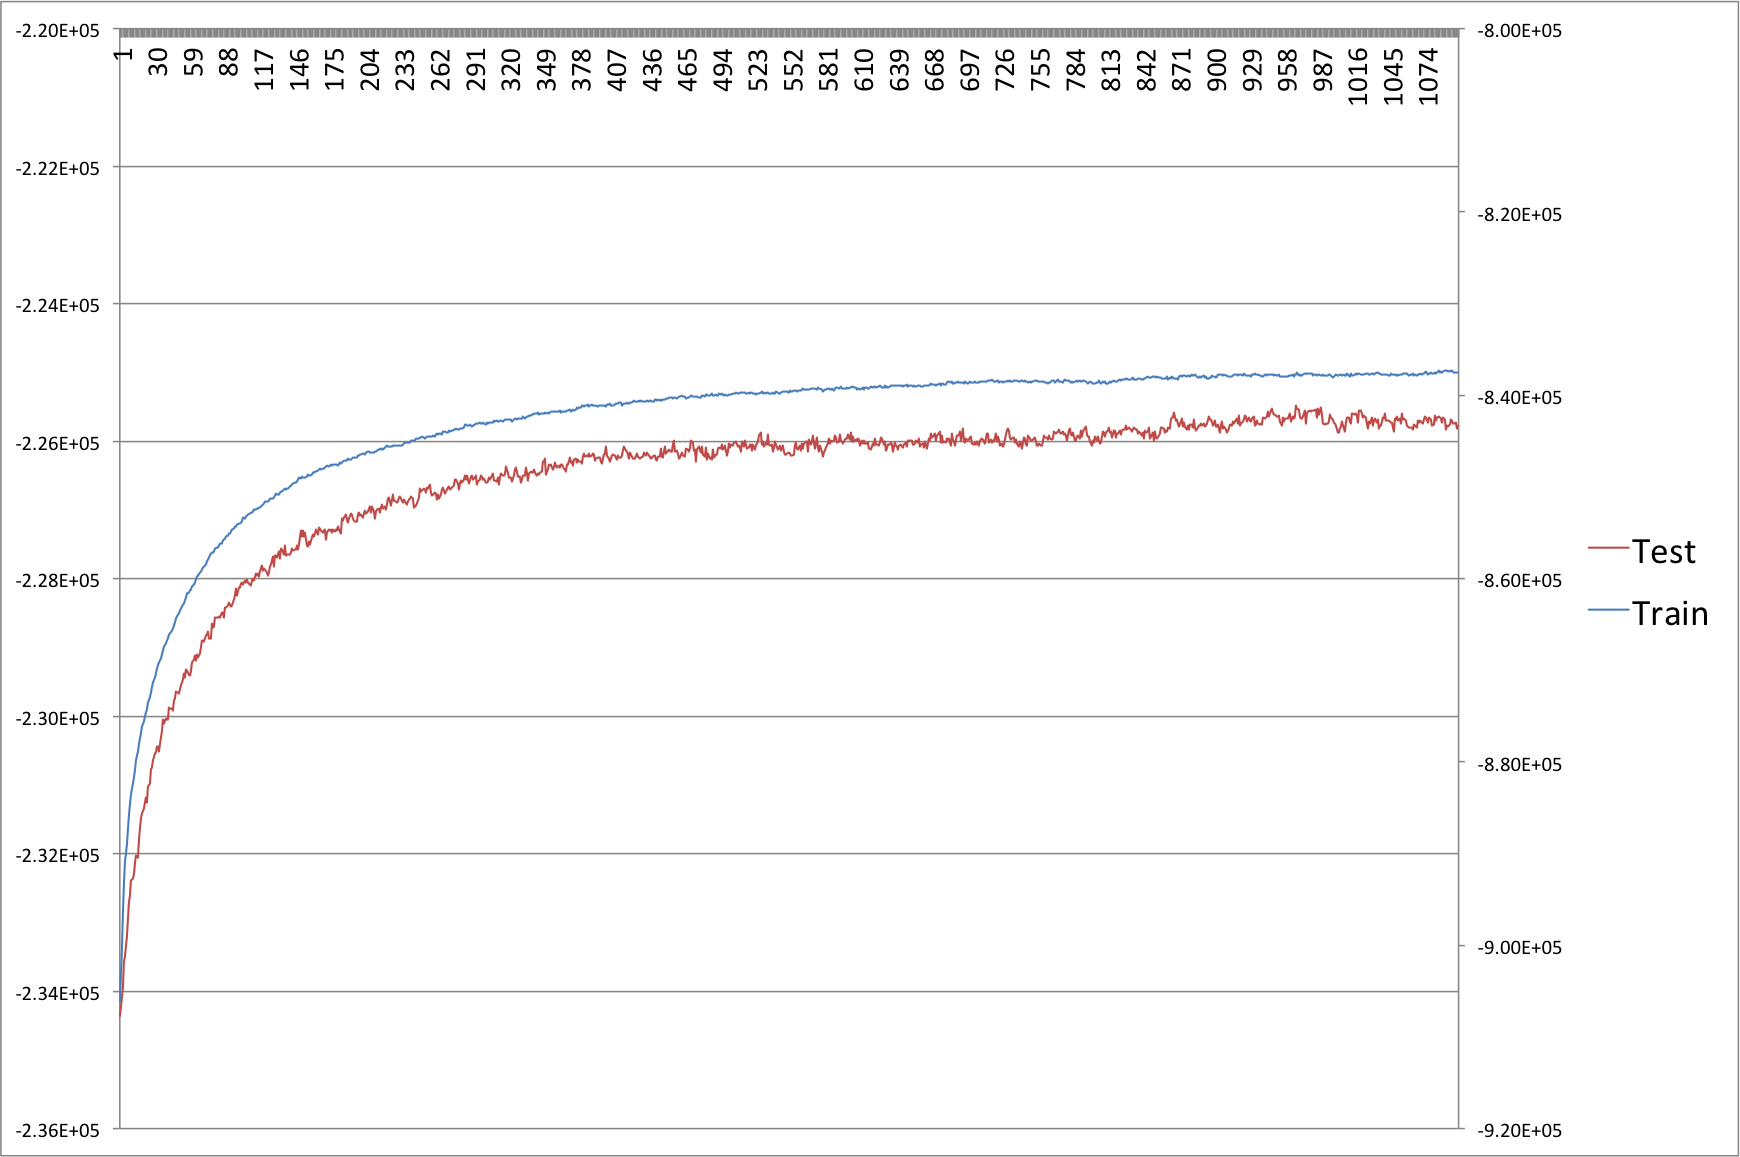
\includegraphics[scale=0.5]{ml_graph_1a}\\
        \end{figure}
        \begin{figure}[ht]
            \caption{Train vs Test data log-likelihood, run 2}
            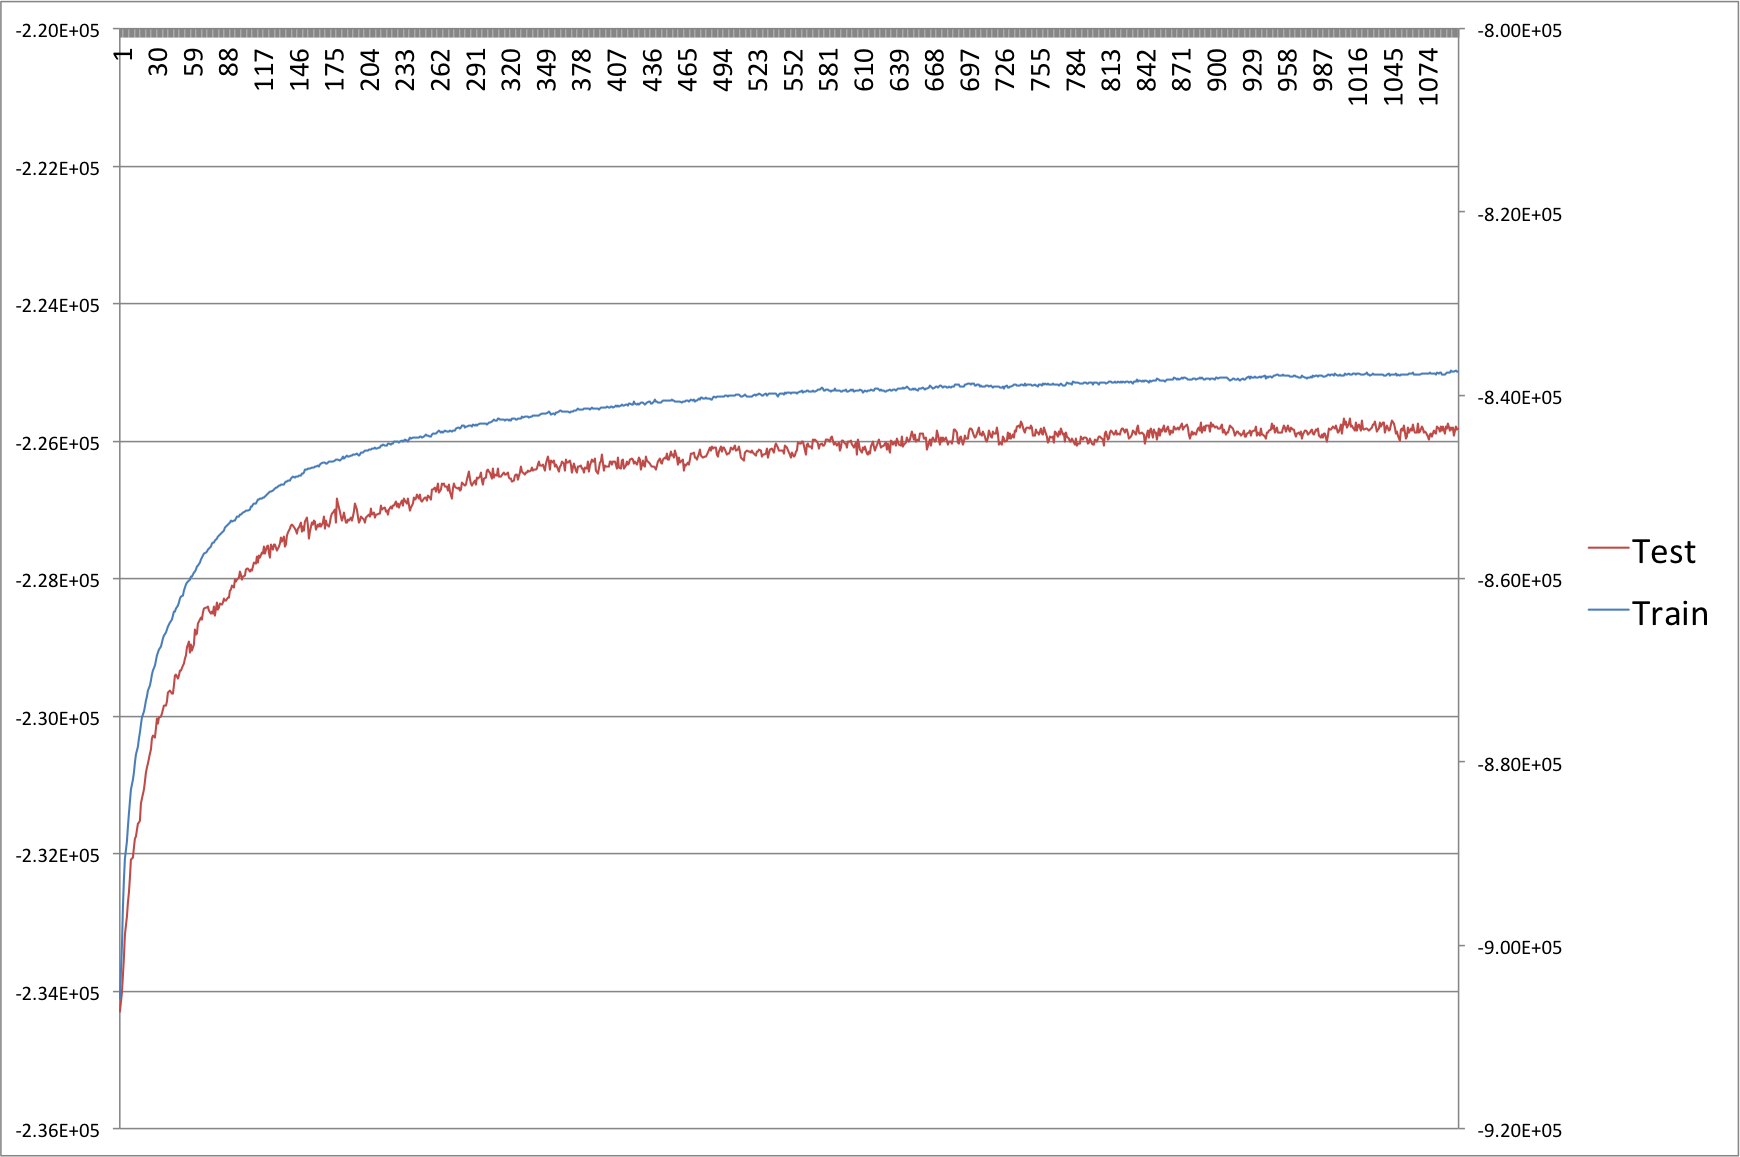
\includegraphics[scale=0.5]{ml_graph_1b}\\
        \end{figure}
        \begin{figure}[ht]
            \caption{Train vs Test data log-likelihood, run 3}
            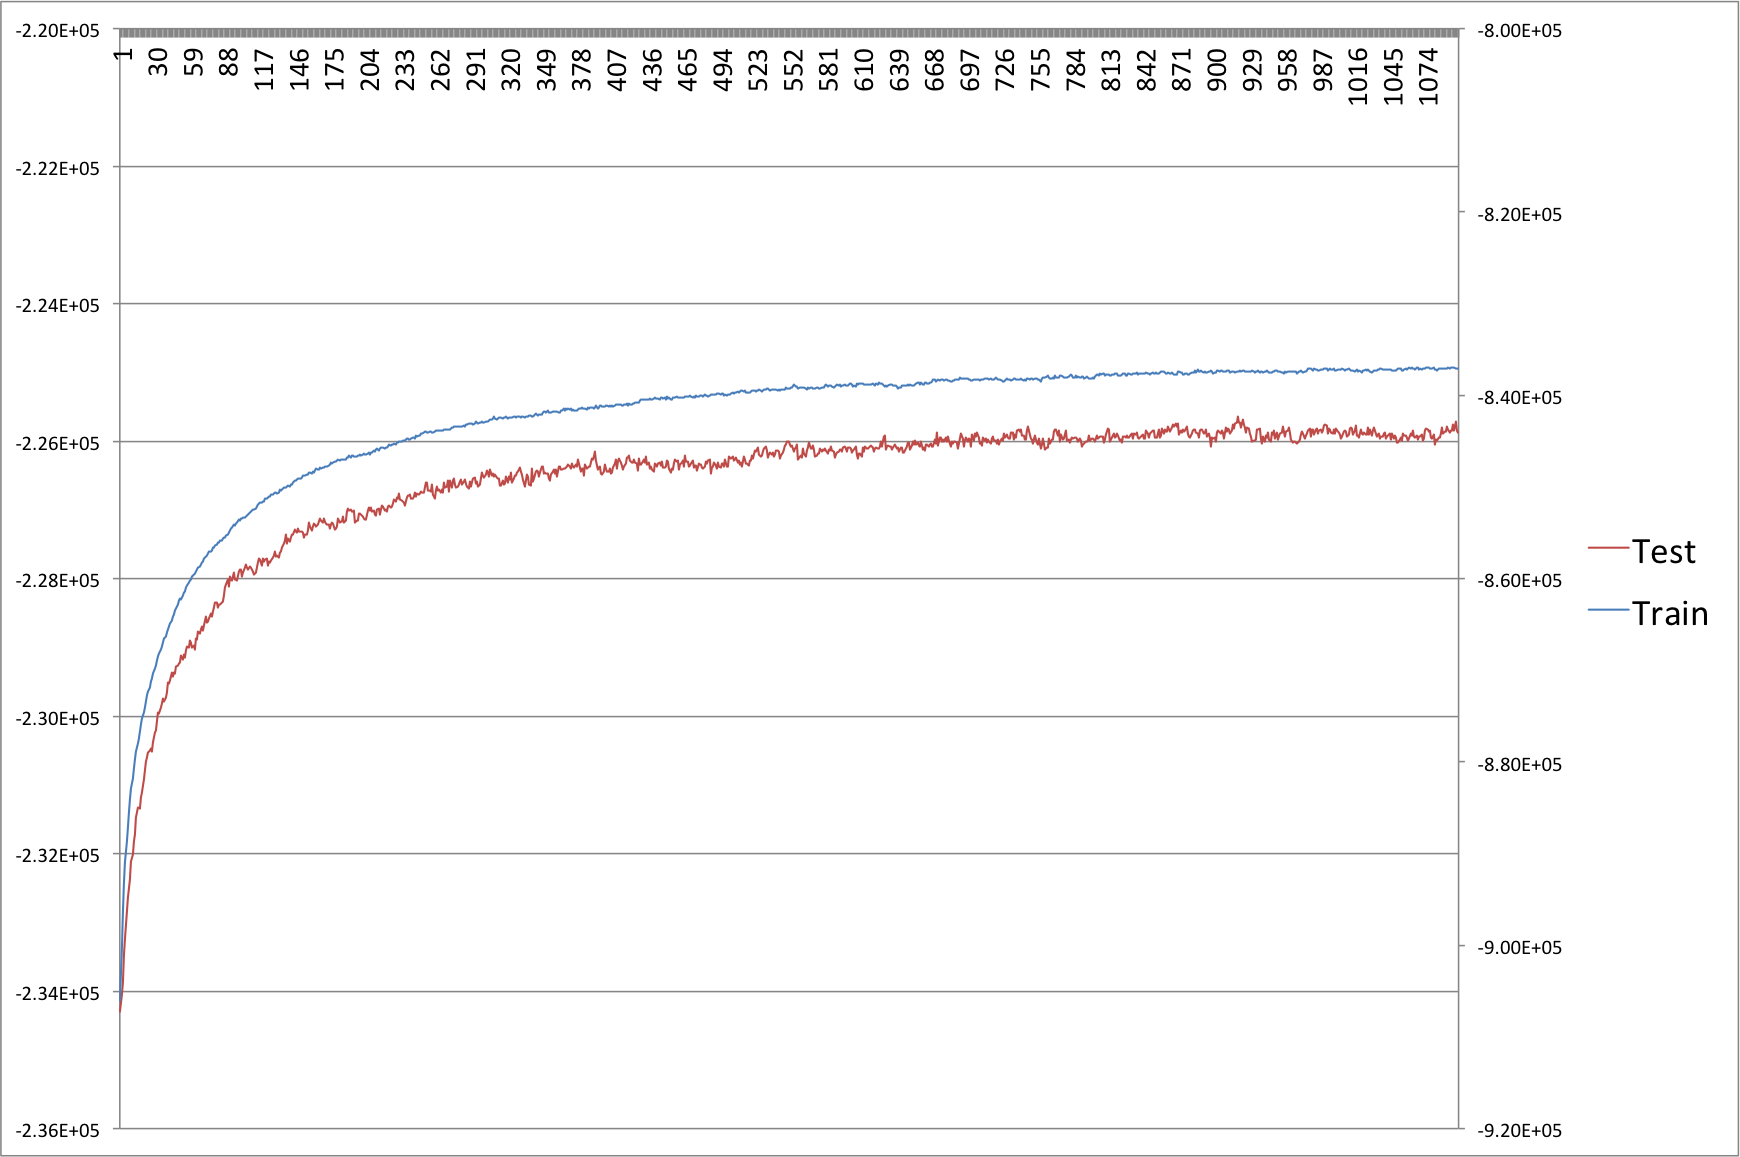
\includegraphics[scale=0.5]{ml_graph_1c}\\
        \end{figure}

    \item 
        The Blocked Gibbs sampler appears to converge much sooner than does the regular Gibbs sampler. We also noticed that the log-likelihood asymptote for Blocked Gibbs was lower than for the Gibbs sampler.

        \begin{figure}[ht]
            \caption{Gibbs sampler vs Blocked Gibbs log-likelihood}
            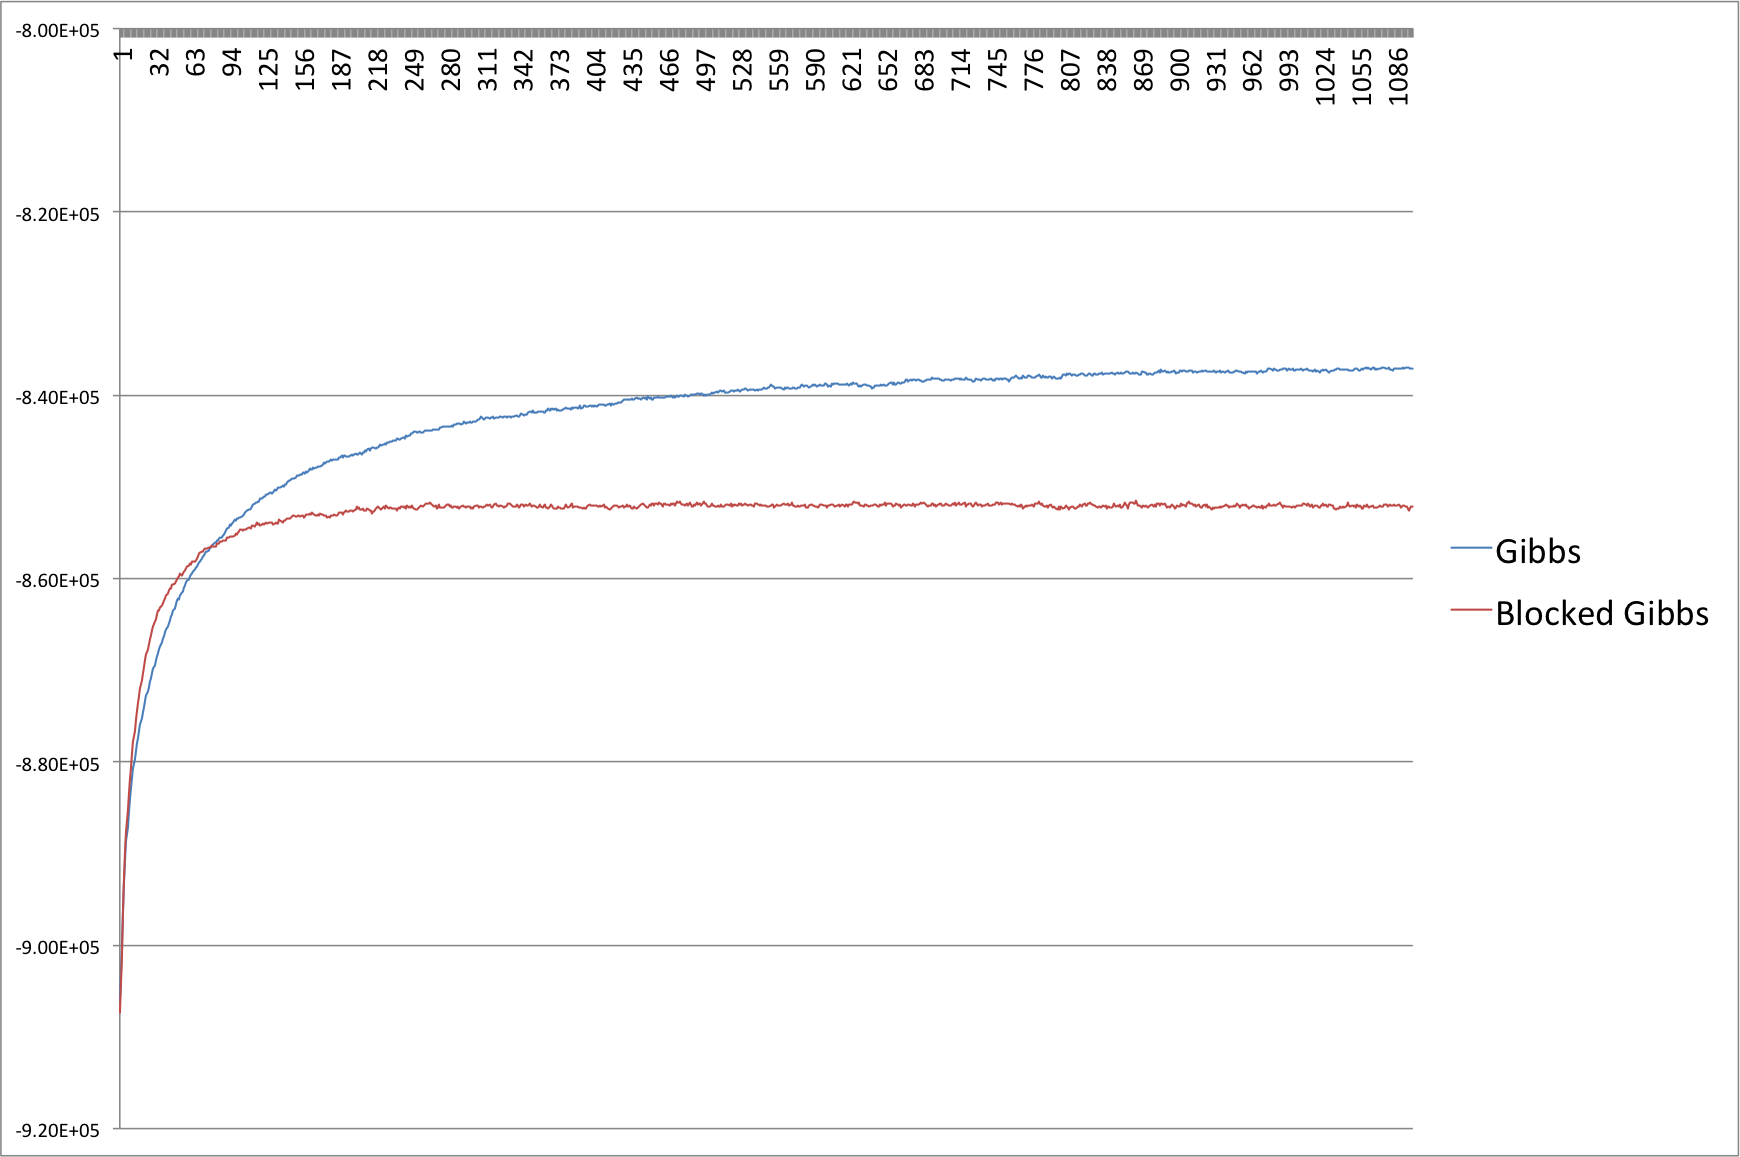
\includegraphics[scale=0.5]{ml_graph_2}\\
        \end{figure}

   \item
       While the Gibbs sampler is faster per iteration, ending its run in almost half the time, the Blocked Gibbs sampler still converges to a stable point much faster, making it more efficient overall.

        \begin{figure}[ht]
            \caption{Gibbs and Blocked Gibbs log-likelihood over time (seconds)}
            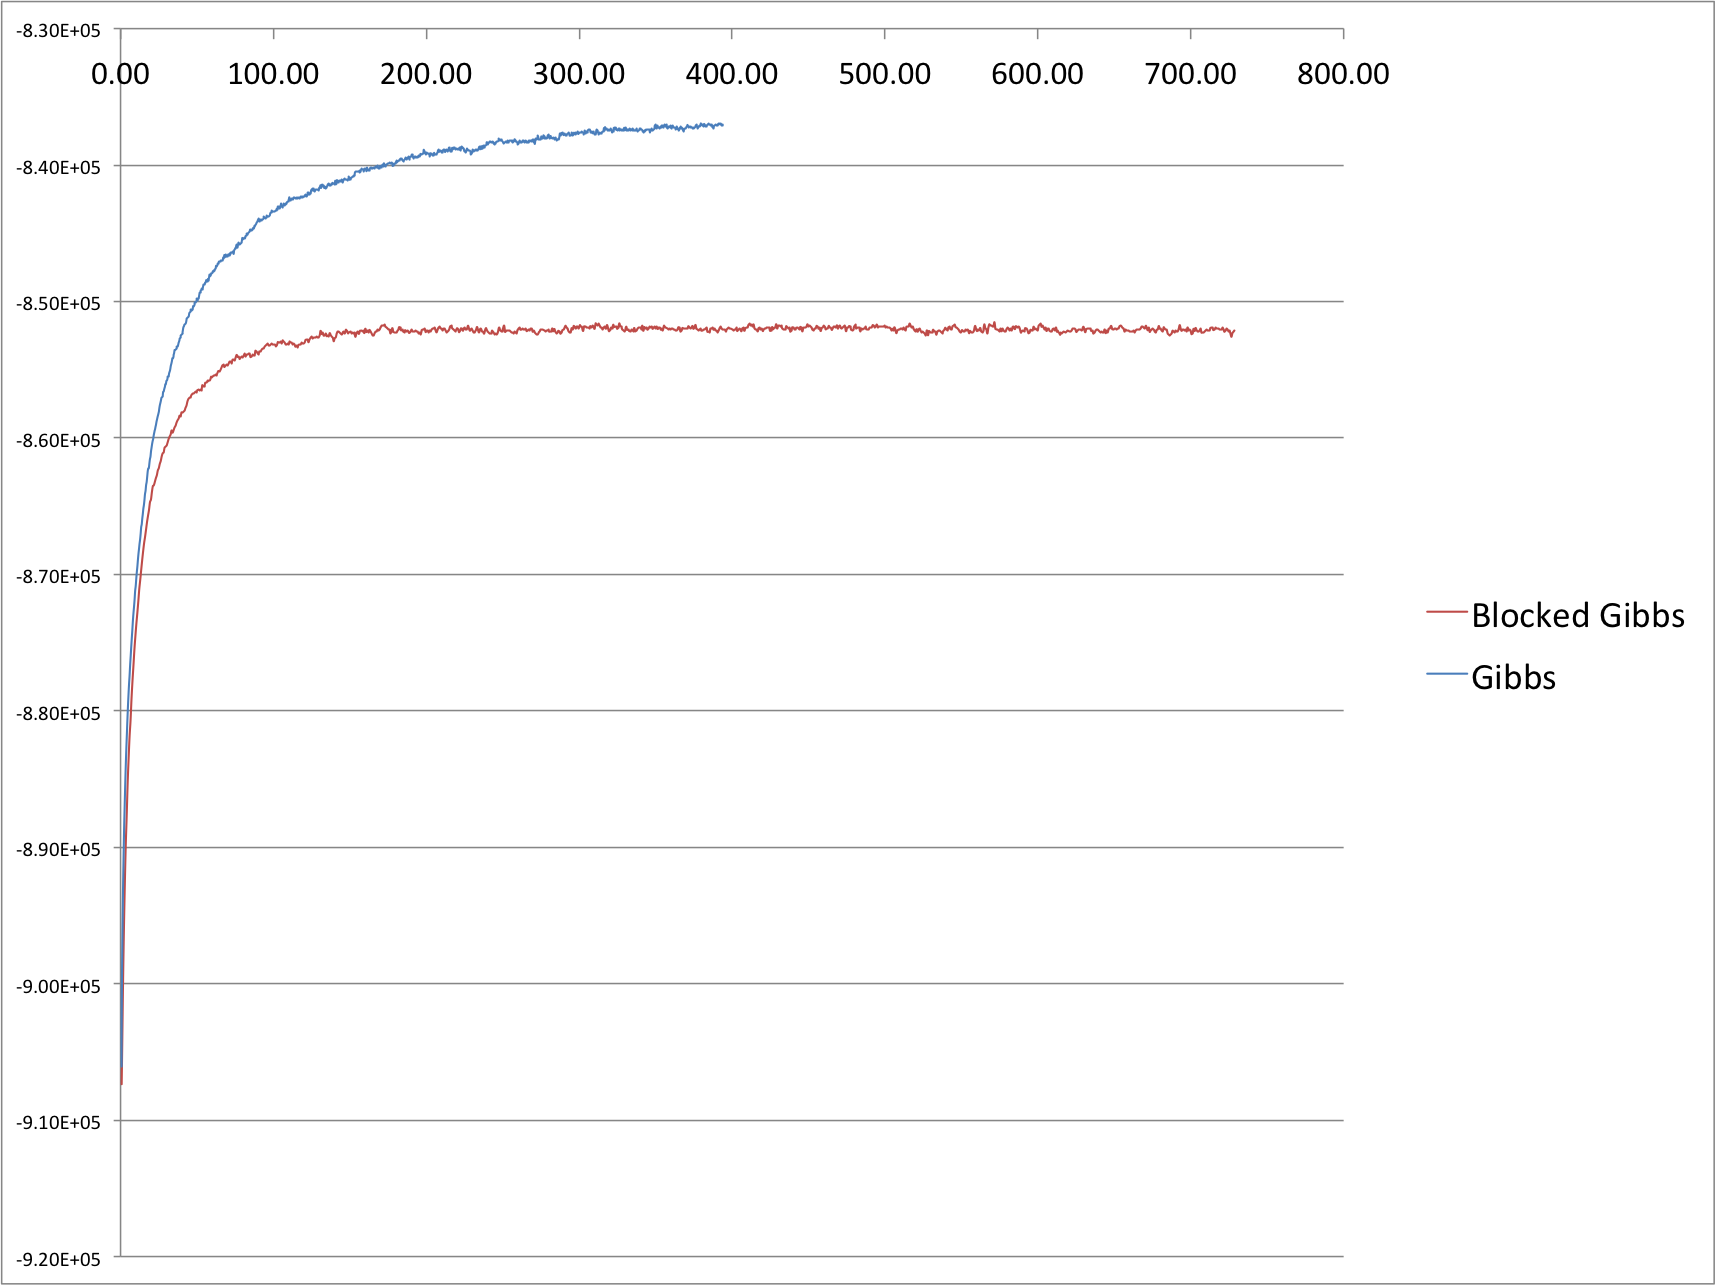
\includegraphics[scale=0.5]{ml_graph_3}\\
        \end{figure}

   \item 
       The test likelihood increases as the number of topics increases.

        \begin{figure}[ht]
            \caption{Test average log-likelihood as a function of topic number}
            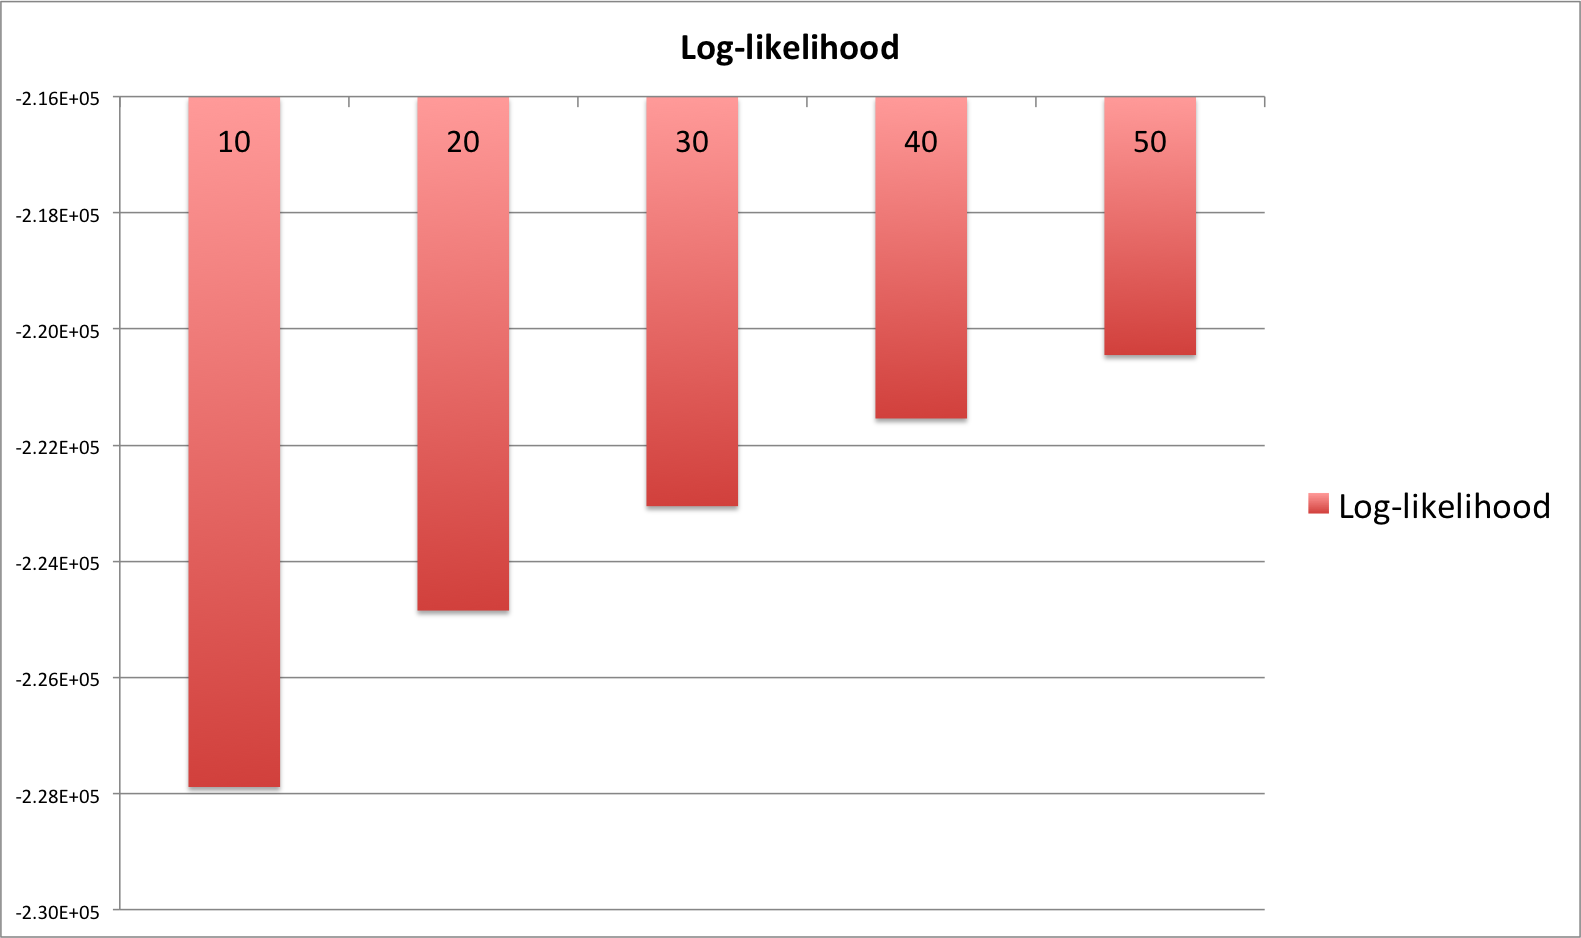
\includegraphics[scale=0.5]{ml_graph_4}\\
        \end{figure}

   \item
       The test likelihood increases as lambda increases.

        \begin{figure}[ht]
            \caption{Test average log-likelihood as a function of $\lambda$}
            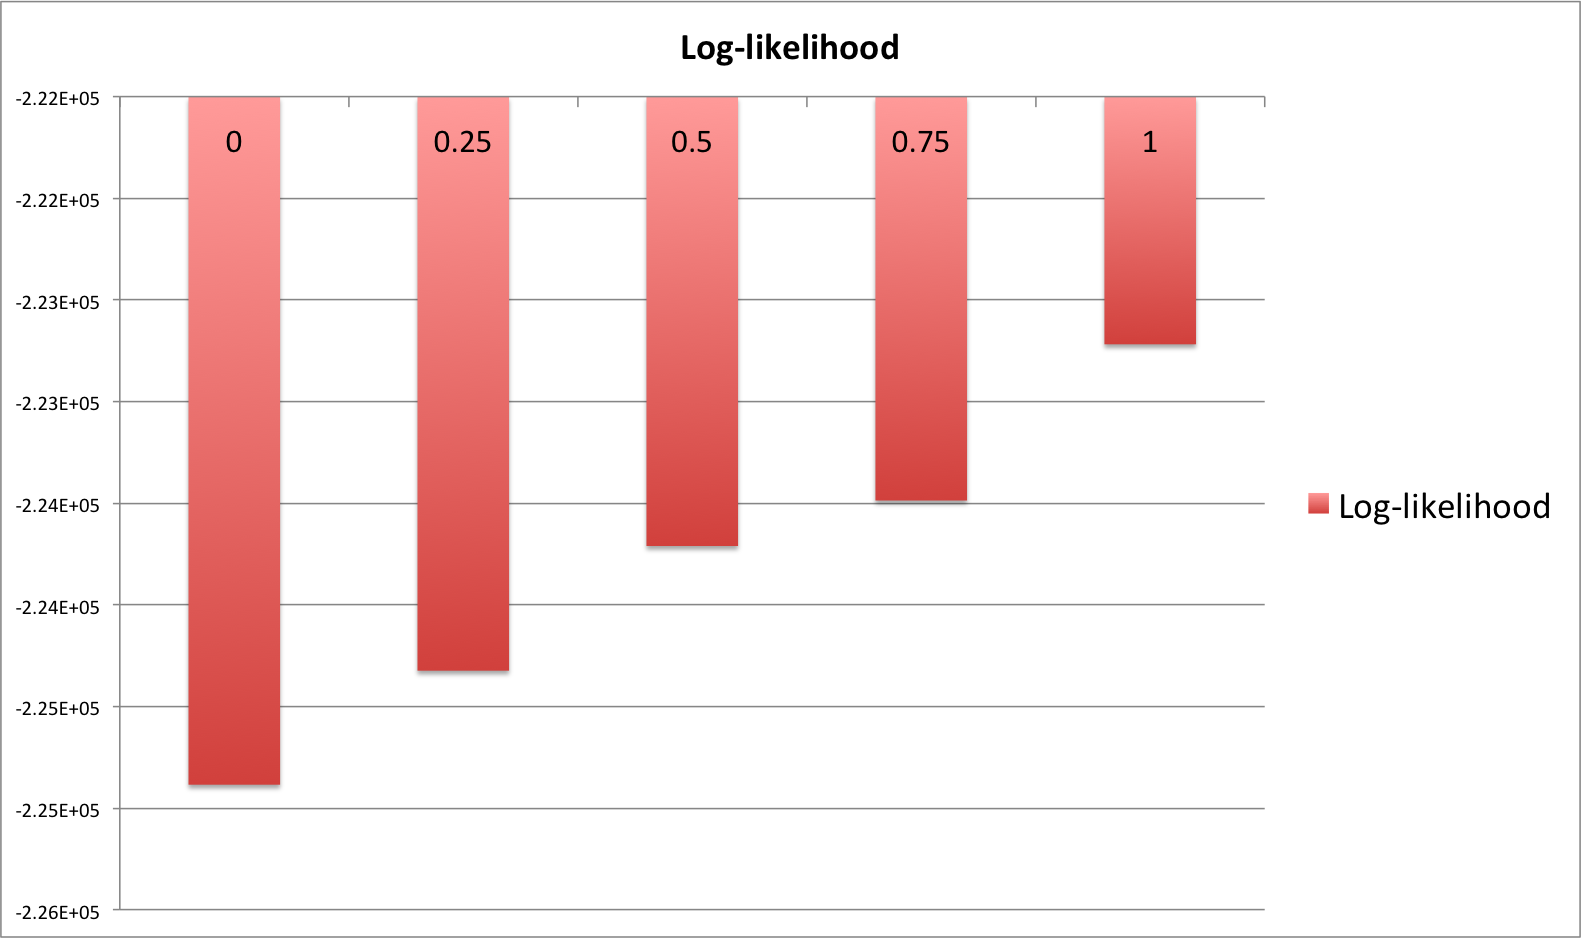
\includegraphics[scale=0.5]{ml_graph_5}\\
        \end{figure}

   \item
      \begin{enumerate}
          \item 
              We tried looking at 25 topics, 10 topics and 5 topics. At the 25 topic level, it was very hard to find any commonality between the corpora. The same is true for the 10 topic level. At the 5 topic level, words like method(s) could sometimes be found in common. However, in general, the global corpus tends to pick words that are \ldots well, general. Words like `input', `model', `paper', that describe scholarship in general but with little specificity were common in the general corpus. On the other hand, the specific corpora picked up on specific topics of machine learning, often separating them neatly into different topics. Corpus 0 specifically splits up into topics to do with machine vision, neural networks, gaussian models, and neuroscience-related topics. Corpus 1 deals almost completely with NLP and text processing. 
              
          \item
              When lambda is close to 0, the global topics dominate, taking all of the data. The specific corpora approach a uniform distribution of low probability of words in every topic. When lambda is close to 1, the opposite happens.

          \item
              When alpha is high, many topics peak on a few top words with very high probability, while the lower ranked words have low probability. When alpha is low, the probabilities are much more uniform. We think this has to do with the fact that a high alpha makes document-specific assignment to topics uniform so that the only effect on topic assignment has to do with word frequency per topic from the beta.

              When beta is high, the topic distributions approach uniformity. When beta is low, the probabilities are not `smoothed out' and vary more.
      \end{enumerate}

\end{enumerate}

\end{document}
